% Session 10 -- the Kohn-Sham self-consistency loop and the two places machine learning enters it.
% Placement: sec. "Machine learning in density functional theory", at the itemized list of
% the two ML strategies.
% Rendered by figures/blender/s10f04_dftml.py, labels in figures/overlays/s10f04_dftml.tex.
\begin{aqmfigure}{fig:s10:dft}{Where machine learning enters density functional theory, and why the
two entry points are different ideas. The Kohn-Sham loop (10.8), the ring in the middle, turns the
problem into a self-consistent single-particle problem. \textbf{Route 1} replaces the unknown
exchange-correlation part by a trained network. This is more accurate, but the diagonalization stays
inside the loop, and the diagonalization, not $v_{\rm xc}$, is what limits the system size.
\textbf{Route 2} learns the Hohenberg-Kohn map $v_{\rm ext}\mapsto n$ directly, trained on
conventional Kohn-Sham results for small systems, and then does no diagonalization at all, so the
whole loop is skipped. Only route 2 changes which systems we can compute, while route 1 only changes
how good the answer is.}
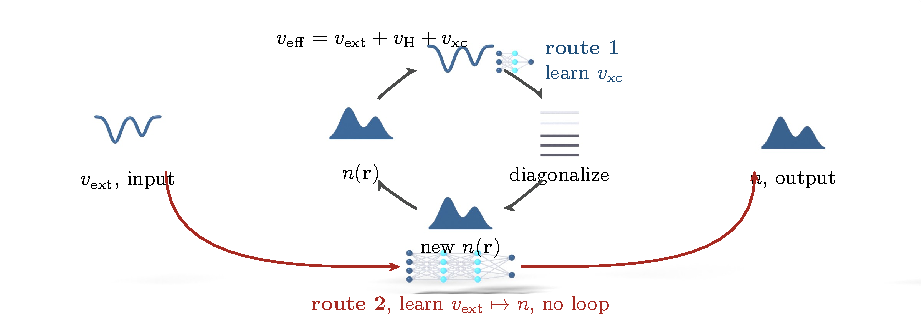
\includegraphics{figures/pdf/s10f04_dftml.pdf}
\end{aqmfigure}
